%Semantics of state charts
\section{Semantics of The State Chart Language}

The semantics used for our project was purposely modelled after UML2. As discussed in section \ref{sec:overviewstatechart} UML2 is essentially standard state charts with extensions added on to describe behaviours in states. The motivation to using UML2 as a basis for our state chart system consists of three primary details. First UML2 is quite well known and popular, this improves the potential acceptance of our tool. Secondly UML2 state chart syntax is more concrete than the other forms of state charts, giving a strong basis to construct our language around. Finally UML2 has the concept of internal activity or internal execution necessary for modelling the behaviour of an actual useful program.

The semantics of our state charts can be expressed mathematically as follows:

\begin{itemize}
	\item \textbf{Q:} A set of states.
	\item \textbf{$\Sigma$:} A set of assignments. $Q \times (v_0,v_1 \in \Sigma \bullet v_0 := v_1)$
	\item \textbf{$\tau$:} A set of transitions. $Q \times E \rightarrow Q$
	\item \textbf{$q_0$:} An initial starting state.
\end{itemize}

The set of states denoted by Q includes the starting state that is $(q_0 \in Q)$. Assignments in our system happen in sequence rather than all at once this method was chosen to allow sequential forumlae to be computed in our system easily. Assignments can be in the form of a constant or an equation. If a series of assignment were found in a single state as follows:

\begin{align}
v_1 := v_0 \label{eqn:assign0} \\ 
v_0 := v_1 \label{eqn:assign1}
\end{align}

We would see that the result $v_1 = v_0$ it is important to note this since generally in state charts it is understood that assignments happen cocurrently in such a case equations \ref{eqn:assign0} and \ref{eqn:assign1} would produce a swap where $v'_1 = 'v_0$ and $v'_0 = 'v_1$. In normal state charts we read assignments such as in equations \ref{eqn:assign0} and \ref{eqn:assign1} as these assignments will take place upon entry of the state. For our semantics however, we read them in a sequential fashion for example: Upon entry of the state, first equation \ref{eqn:assign0} is assigned, then \ref{eqn:assign1} right afterwards.

\begin{figure}[htp]
    \centering
    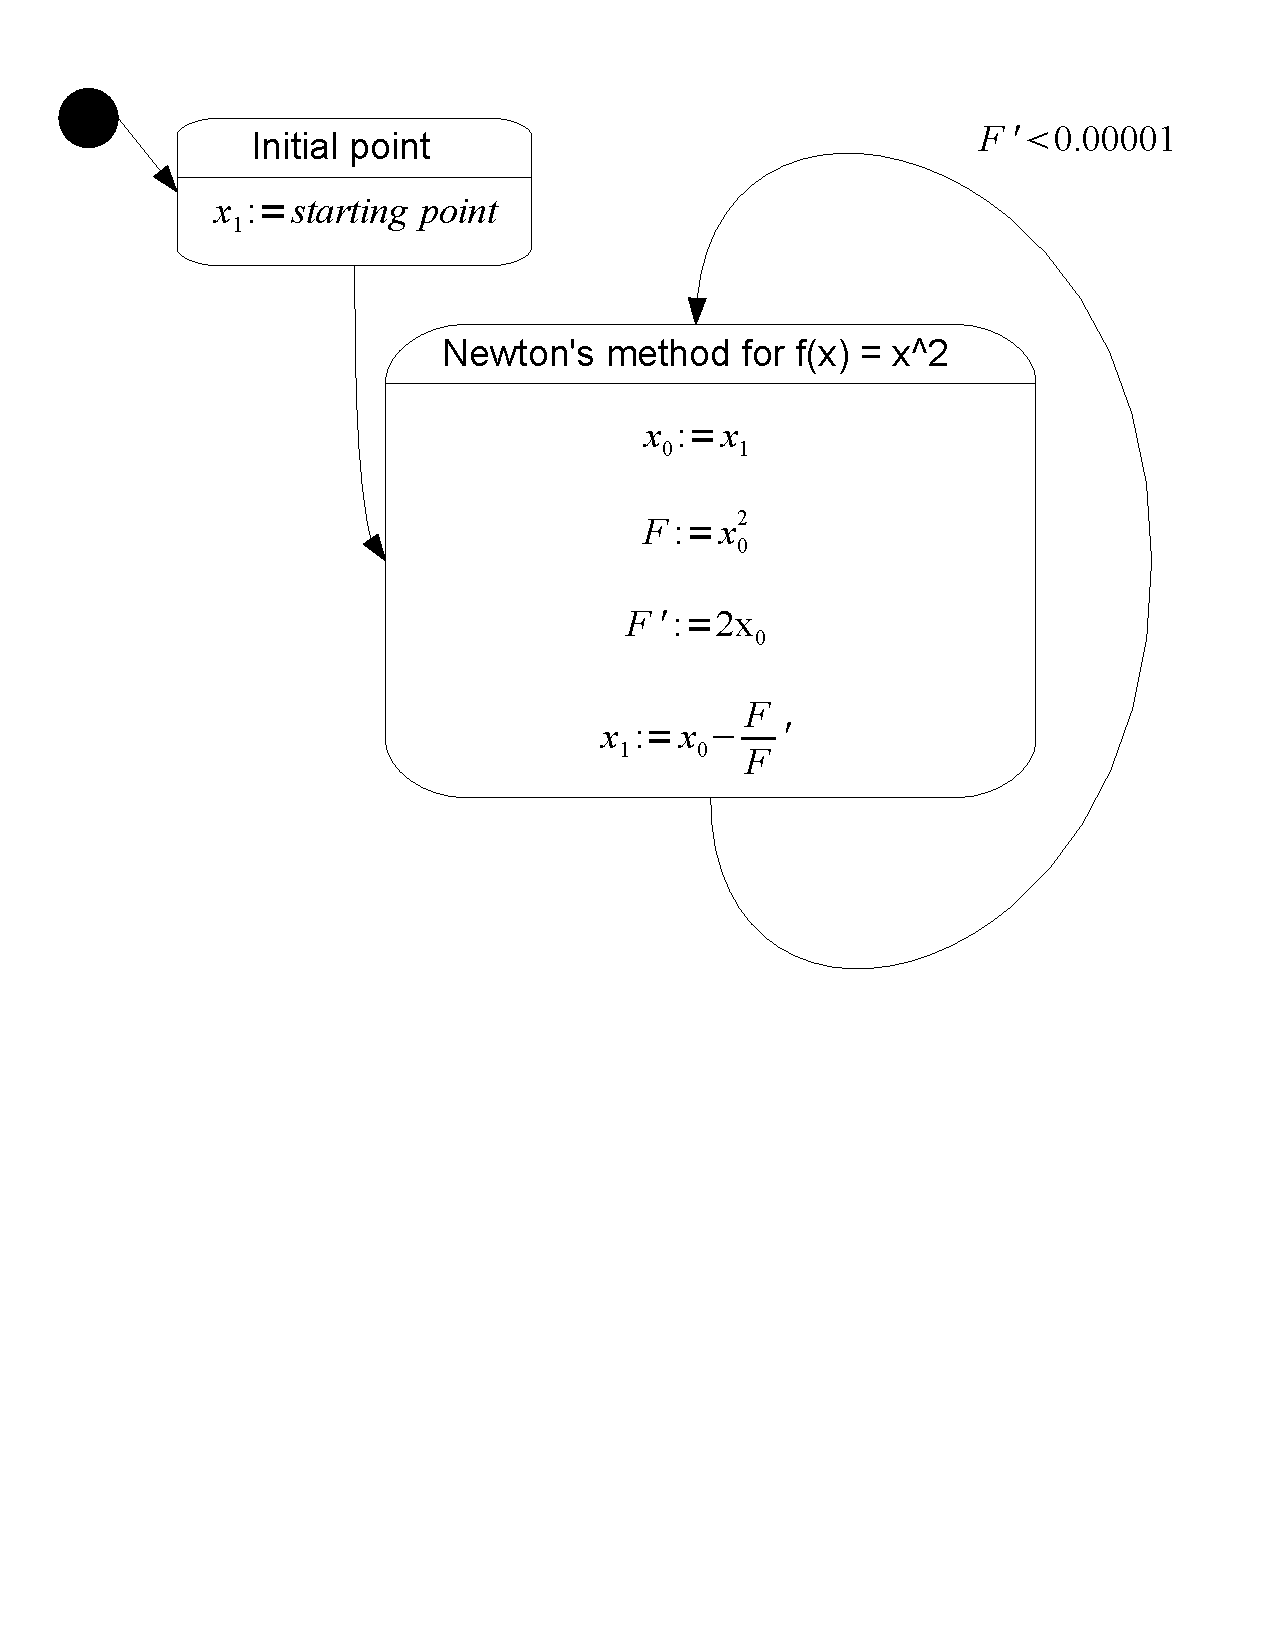
\includegraphics[trim= 10mm 110mm 10mm 10mm, clip, width=\imgmedium]{./images/state_uml2_newtons.pdf}
    \caption{Newton's Method Approximation}
    \label{fig:state_uml2_newtons}
\end{figure}

The advantage of sequential assignments over cocurrent assignments can be seen when trying to compute more complicated formulas as seen in figure \ref{fig:state_uml2_newtons}. Figure \ref{fig:state_uml2_newtons} computes the newton's approximation of $x^2$ given a starting point. If the same formula was to be computed with cocurrent assignments many more states would be required. Thus although this choice slightly deviates from UML2 state charts it was decided the benefits to usability was too great to strictly adhere to the UML2 semantics.

\begin{figure}[htp]
    \centering
    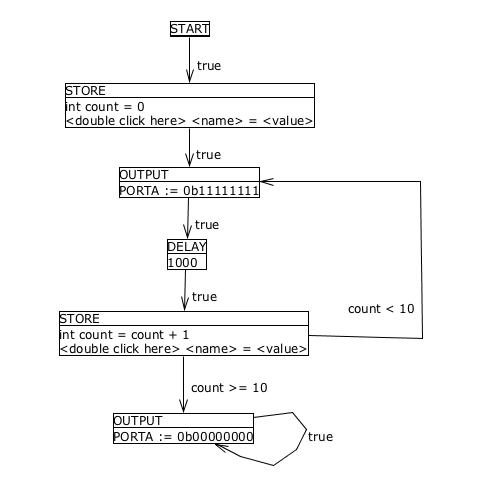
\includegraphics[width=\imgmedium]{./images/tool_transition_example.png}
	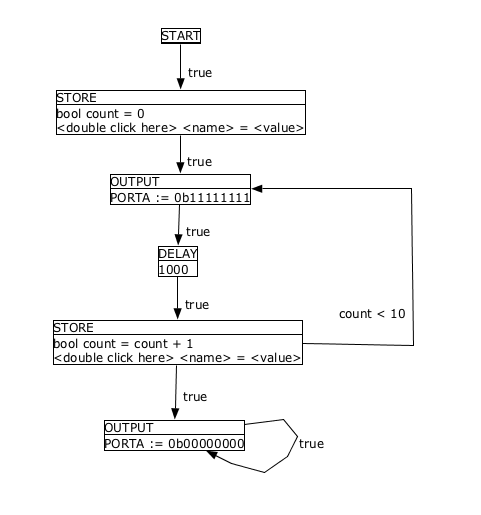
\includegraphics[width=\imgmedium]{./images/tool_transition_example_bad.png}
    \caption{PLC Edit Valid vs Invalid Transitions}
    \label{fig:tool_transition_example}
\end{figure}

Transitions in the language must be mutually exclusive that is if it is invalid to have two transitions that can both be taken at any point. If this does occur 